\chapterimage{Water1}
\chapter{Water Properties and Sources}





\begin{table}[H]
\begin{tabular}{| m{1cm} | m{15cm} |}
\hline
\multicolumn{2}{|l|}{\textbf{Expected   Range of Knowledge for Water Properties and Sources}}                                                                          \\ \hline
\multicolumn{2}{|l|}{\textit{Water   Distribution System Operator License Exams}}                                                                                      \\ \hline
D1 & Ability to measure   well depth                                                                                                   \\ \hline
D1 & Ability to recognize   potential sources of contamination                                                                         \\ \hline
D1 & Knowledge of the   hydrologic cycle                                                                                               \\ \hline
D1 & Knowledge of security   procedures/measures                                                                                       \\ \hline
D1 & Ability to calculate   draw down                                                                                                  \\ \hline
D1 & Ability to recognize   abnormal pH levels of water in a distribution system                                                       \\ \hline
D1 & Ability to recognize   abnormal turbidity levels in a distribution system                                                         \\ \hline
D1 & Knowledge of normal   pH range in drinking water                                                                                  \\ \hline
D1 & Knowledge of the   impacts of high nitrate concentrations in a distribution system                                                \\ \hline
D1 & Knowledge of the   meaning of high levels of turbidity in a distribution system                                                   \\ \hline
D1 & Knowledge of   contamination sources in a well                                                                                    \\ \hline
D1 & Knowledge of water   storage contamination sources                                                                                \\ \hline
D1 & Ability to measure   the water depth in a well                                                                                    \\ \hline
D1 & Knowledge of water   depth measurement techniques                                                                                 \\ \hline
D2 & Knowledge of cone of   depression                                                                                                 \\ \hline
D2 & Knowledge of recovery   time                                                                                                      \\ \hline
D2 & Knowledge of static   and pumping water level                                                                                     \\ \hline
D2 & Knowledge of water   table fluctuations                                                                                           \\ \hline
D2 & Knowledge of well   components and terms                                                                                          \\ \hline
D2 & Knowledge of well   protection                                                                                                    \\ \hline
D2 & Knowledge of zone of   influence                                                                                                  \\ \hline
D2 & Knowledge of proper   installation of a sanitary seal on a well                                                                   \\ \hline
D3 & Knowledge of the   vulnerability assessment                                                                                       \\ \hline
D3 & Knowledge of well   location requirements                                                                                         \\ \hline
D3 & Knowledge of the   chemical components of groundwater                                                                             \\ \hline
D3 & Ability to calculate   specific yield                                                                                             \\ \hline
\end{tabular}
\end{table}

\newpage



\begin{table}[H]
\begin{tabular}{| m{1cm} |m{15cm} |}
\hline
\multicolumn{2}{|l|}{\textbf{Expected   Range of Knowledge for Water Properties and Sources}}                                                                      \\ \hline
\multicolumn{2}{|l|}{\textit{Water   Distribution System Operator License Exams (Continued)}}                                                                  \\ \hline
D4 & Knowledge of long-term water availability                                                                                         \\ \hline
D4 & Knowledge of sanitary survey requirements                                                                                         \\ \hline
D4 & Knowledge of the characteristics of   aquifers                                                                                    \\ \hline
D4 & Knowledge of proper gravel packing and   screen depth                                                                             \\ \hline
D4 & Knowledge of well abandonment procedures and   permit requirements                                                                \\ \hline
D4 & Ability to estimate future water needs                                                                                            \\ \hline
D4 & Knowledge of capital improvement/capital   replacement requirements                                                               \\ \hline
D5 & Knowledge of permit   requirements                                                                                                \\ \hline
\multicolumn{2}{|l|}{\textit{Water   Treatment System Operator License Exams}}                                                                  \\ \hline
T1 & Ability to recognize   abnormal well operations                                                                                   \\ \hline
T1 & Ability to recognize   potential security risks                                                                                   \\ \hline
T1 & Ability to recognize   potential sources of contamination in surface water                                                        \\ \hline
T1 & Ability to recognize   the influence of surface water on a groundwater source                                                     \\ \hline
T1 & Knowledge of flow   measurement devices                                                                                           \\ \hline
T1 & Knowledge of   potential microbial and chemical contamination sources in groundwater and   surface water                          \\ \hline
T1 & Knowledge of the   characteristics of aquifers                                                                                    \\ \hline
T1 & Knowledge of the   hydrologic cycle                                                                                               \\ \hline
T1 & Knowledge of visual   signs of contamination in a surface water reservoir                                                         \\ \hline
T1 & Knowledge of well   components                                                                                                    \\ \hline
T1 & Knowledge of well   depth measurement procedures                                                                                  \\ \hline
T1 & Knowledge of well   disinfection procedures                                                                                       \\ \hline
T1 & Knowledge of well   drawdown measurement techniques                                                                               \\ \hline
T1 & Knowledge of   waterborne pathogens                                                                                               \\ \hline
T1 & Ability to interpret   water quality reports                                                                                      \\ \hline
T2 & Ability to   discriminate between normal and abnormal conditions of a surface water   reservoir                                   \\ \hline
T2 & Ability to recognize   hydrological changes                                                                                       \\ \hline
T2 & Knowledge of how   reservoir intake level effects water quality                                                                   \\ \hline
T2 & Knowledge of the   effects of seasonal changes on water reservoirs                                                                \\ \hline
T3 & Knowledge of surface   water reservoir stratification                                                                             \\ \hline
T3 & Ability to recognize   head loss across an intake screen                                                                          \\ \hline
T3 & Knowledge of   groundwater treatment procedures                                                                                   \\ \hline

T4 & Ability to interpret historical water use data                                                                                   \\ \hline
\end{tabular}
\end{table}

\newpage







































\section{Properties of water}\index{Properties of water}
\begin{itemize}
\item Water is one of the most abundant and common materials on earth. It covers 70 percent of the surface of the earth as water and ice.
\item Water makes up 60-75\% of human body weight. A loss of just 4\% of total body water leads to dehydration, and a loss of 15\% can be fatal.
\item A person could survive a month without food but would not survive 3 days without water \index{Human body component}.
\item Even though most other planets have water in some form, the earth is the only planet in the solar system that contains water in all its common forms (gas, liquid, solid).  Others have ice, but only the earth has an abundance of this miraculous substance in the proper temperature range to support life.
\item Its chemical formula, H$_2$O, indicates that each of its molecules contains one oxygen and two hydrogen atoms.  
\item The much larger oxygen atom is connected by covalent bonds to each of the two hydrogen atome. The hydrogen atoms are attached to the oxygen atom at an angle of 104.45\si{\degree}.
\item Even though the water molecule is overall neutral, its bent shape results in the accumulation of positive charge near the oxygen end and negative charge near the hydrogen.  This differential in charges makes the water molecule \textbf{polar} \index{Polar} - like a magnet and bestows it unique properties. 
\item The polarity and molecule size of water imparts it a unique property of being able to dissolve a very wide range of minerals, chemicals and gases which makes it indispensable for the existence of lifeforms and a very critical element of our day-to-day life.  However, many of the substances dissolved in water must be removed during treatment to make water safe to drink.
\item Nonpolar substances such as oils, fats, and many organic compounds do not dissolve as easily in water.
\begin{figure}[h]
\begin{center}
        \includegraphics[scale=0.25]{WaterMolecule}
        \caption{Water molecule}
        \label{Water molecule}
\end{center}
\end{figure}
\vspace{0.5cm}

\item Pure water will not conduct electrical current. But when soluble salts such as sodium chloride (NaCl), calcium carbonate (CaCO$_3$) are present in water, water will conduct electricity as these salts ionize - break into its constituent positive and negative charged particles the water, and the charged ions make water to conduct electrical current.
$$NaCl \leftrightarrow Na^+ + Cl^-$$
\item The more ions there are in a solution, the more easily the current flows. The ability to conduct electrical current is called conductivity and can be used to indirectly estimate the amount of total dissolved solids in the water.\\
\item The boiling of water - 100\si{\degree}C or 212\si{\degree}F and its melting/freezing point - 0\si{\degree}C or 32\si{\degree}F is very high  compared to similar molecules and it is the only natural substance found in all three physical states at the temperatures that naturally occur on Earth.
\item Most other substances become more dense as they cool.  However, ice is less dense than water which makes ice float on water.
\item Ice on the water surface insulates the water below preventing it from freezing and allowing for fish and other life form to survive and allows for the movement of animals who live in these cold habitats.
\item As water cools, its density increases upto 4\si{\degree}C after which it gets less dense as it is cooled further.
\item The changing density of water is responsible for turnover of a lake during fall.  When the surface water cools, the cold water becomes more dense than the warm water below so the cold water sinks to the bottom and warm water rises to the top.  When lakes are used as the source water for water treatment plants, turnover can cause abrupt changes in the quality of raw water.
\item It needs a lot of energy to make the water warmer or cooler (high Specific Heat) which allows for keeping the temperature of water bodies such as oceans, rivers, ponds more or less constant despite the heat from the sun.
\item Water molecules stick together well because of its high surface tension - which allows for water to rise up in tubes through capillary action.  This capillary action allows for plants to draw water along with nutrients from the ground.
\end{itemize}


\section{Water use}\index{Water use}
\begin{itemize}
\item Besides it being needed for basic sustenance of all living beings, water is vital element for the world economy and sustenance of the human society in various ways including:
\begin{itemize}
\item As a food source - fishing
\item For commerce - shipping, trade and transportation
\item For recreation - swimming, skiing, surfing etc.
\end{itemize}
\item Breakdown of global freshwater use:\\
70\% is used for agriculture\\
19\% is used by industries, and \\
11\% is for municipal use
\end{itemize}

\section{Water supplies}\index{Water supplies}
\begin{itemize}
\item Civilizations have always formed near water sources - on the banks of rivers. Ancient Egyptians - on the Nile, Mesopotamians in the Fertile Crescent on the Tigris/Euphrates rivers, Ancient Chinese on the Yellow River, and the Ancient India on the Indus.
\item The water on our Earth today is the same water that has been here for nearly 5 billion years.\\
\item Water molecules were formed in interstellar space by chemical reactions between hydrogen molecules and oxygen-bearing molecules such as carbon monoxide and the Earth inherited its water from asteroids and comets crashing into it.
\item The only thing that changes is the form that water takes as it travels through the water cycle.
\item On Earth, water is the only substance that can occur naturally in its three states of matter -  gas, liquid and solids, circulates naturally through its five principal realms:
\begin{itemize}
\item Oceans
\item Atmosphere
\item Lakes and rivers
\item Icecaps and glaciers
\item Underground
\end{itemize}
This is the planetary Water Cycle. \index{Water cycle}
\item Elements of the water cycle include:
\begin{itemize}
\item Transpiration - process by which plants lose water as vapor out of their leaves. 
\item Evaporation - conversion of water in oceans, rives and lakes into vapor by the heat from the sun
\item Evapotranspiration is the combined processes of evaporation and transpiration - the movement of water from oceans or land to the atmosphere.
\item Condensation - cooling of water vapor in the upper layer of earths atmosphere into liquid water in the form of clouds
\item Precipitation - discharge of the water bearing clouds as rain, hail, sleet or snow.
\item Infiltration - movement of water from surface to soil.
\end{itemize} 
\item Life on earth is dependent on the Earth's water cycle \index{Water cycle}
\begin{figure}[]
\begin{center}
\includegraphics[scale=0.8]{Watercycle1}\index{Water cycle}
\caption{Water cycle}
\label{Water cycle}
\textit{(Credit:David Cain/NWS)}
\end{center}
\end{figure}
\item A watershed \index{Watershed} is the area of land, where all of the water that falls in it and drains off of it into to a common outlet which could be a one or combination of water bodies such as a river, lake or underlying groundwater.
\item The natural features including - mountains, trees, shrubs, grasses, and man-made features such as urban area, industries, wastes and water discharges affect the quality of the water in or from the watershed.
\item Watersheds are important sources of drinking water, as well as a habitat for many aquatic species. Healthy watersheds with intact native vegetation and wetlands provide important functions such as water purification, flood control, nutrient recycling, and groundwater recharge.
\item Water covers about 71\% of Earth's surface.  The distribution of Earth's water \index{Distribution of earth's water} is provided in the below table.

% Please add the following required packages to your document preamble:
% \usepackage{multirow}
\begin{table}[ht]
\begin{center}
\begin{tabular}{|l|l|llll}
\hline
\multirow{9}{*}{Fresh water} & \multirow{9}{*}{2.50\%} & \multicolumn{1}{l|}{\multirow{7}{*}{Surface water}} & \multicolumn{1}{l|}{\multirow{7}{*}{1.20\%}} & \multicolumn{1}{l|}{Atmosphere}                & \multicolumn{1}{l|}{3.00\%}  \\ \cline{5-6} 
                             &                         & \multicolumn{1}{l|}{}                               & \multicolumn{1}{l|}{}                        & \multicolumn{1}{l|}{Living things}             & \multicolumn{1}{l|}{0.26\%}  \\ \cline{5-6} 
                             &                         & \multicolumn{1}{l|}{}                               & \multicolumn{1}{l|}{}                        & \multicolumn{1}{l|}{Rivers}                    & \multicolumn{1}{l|}{0.49\%}  \\ \cline{5-6} 
                             &                         & \multicolumn{1}{l|}{}                               & \multicolumn{1}{l|}{}                        & \multicolumn{1}{l|}{Swamps, marshes}           & \multicolumn{1}{l|}{2.60\%}  \\ \cline{5-6} 
                             &                         & \multicolumn{1}{l|}{}                               & \multicolumn{1}{l|}{}                        & \multicolumn{1}{l|}{Soil moisture}             & \multicolumn{1}{l|}{3.80\%}  \\ \cline{5-6} 
                             &                         & \multicolumn{1}{l|}{}                               & \multicolumn{1}{l|}{}                        & \multicolumn{1}{l|}{Lakes}                     & \multicolumn{1}{l|}{20.90\%} \\ \cline{5-6} 
                             &                         & \multicolumn{1}{l|}{}                               & \multicolumn{1}{l|}{}                        & \multicolumn{1}{l|}{Ground ice and permafrost} & \multicolumn{1}{l|}{69.00\%} \\ \cline{3-6} 
                             &                         & \multicolumn{1}{l|}{groundwater}                   & \multicolumn{1}{l|}{30.10\%}                 &                                                &                              \\ \cline{3-4}
                             &                         & \multicolumn{1}{l|}{Glaciers and ice caps}          & \multicolumn{1}{l|}{68.70\%}                 &                                                &                              \\ \cline{1-4}
Other saline   water         & 0.90\%                  &                                                     &                                              &                                                &                              \\ \cline{1-2}
Oceans                       & 96.50\%                 &                                                     &                                              &                                                &                              \\ \cline{1-2}
\end{tabular}
\caption{Distribution of earth's water} \index{Earth's water} \label{Earth's water}
\textit{(From:  Igor Shiklomanov's chapter "Worlds fresh water resources" in Peter H. Gleick (editor), \\1993, Water in Crisis: A guide to the world's Fresh water resources)}
\end{center}
\end{table}

\begin{figure}[]
\begin{center}
\includegraphics[scale=0.5]{EarthsWater}
\caption{Distribution of earth's water} \index{Distribution of earth's water} \label{Distribution of earth's water}
\textit{(From:  Igor Shiklomanov's chapter "Worlds fresh water resources" in Peter H. Gleick (editor), \\1993, Water in Crisis: A guide to the world's Fresh water resources)}
\end{center}
\end{figure}

\item 97\% of the Earth's water can be found in our ocean and freshwater is only 2.5\% of all the water on earth
\item Most of the fresh water is in form of ice in glaciers, ice caps and permafrost.  
\item A very very small fraction - about 0.006\% of the total water is the freshwater in lakes and rivers.  Most of the remaining freshwater is in groundwater - about 0.75\% of the total water or about 30\% of the total freshwater.
\item Clean water is vital to our health, communities, and economy. 
\item There is no universally accepted definition of “safe drinking water.” Generally speaking, safe drinking water, is defined as the water that does not represent any significant risk to health over a lifetime of consumption.
\item Water scarcity can be caused by a mix of hydrological, infrastructural, political and social issues. 
\item In developing countries, water supply and sanitation related factors cause more than 20 percent of deaths of people under age 14. Nearly
half of all people in developing countries have infections or diseases associated with inadequate water supply and sanitation.
\item Chemical contaminants in drinking water arise including arsenic, fluoride or nitrate, emerging contaminants such as pharmaceuticals, pesticides, per- and polyfluoroalkyl substances (PFASs) and microplastics generate public concern.
\item Microbiologically contaminated drinking water can transmit diseases such as diarrhoea, cholera, dysentery, typhoid and polio and is estimated to cause 485 000 diarrhoeal deaths each year.
\item The amount of water that is available for sustenance including agriculture, sanitation and hygiene is limited in many areas of the world.  Billions of people throughout the world are battling daily against enormous difficulties accessing the most basic services.\\
\item Some 1.1 billion people worldwide lack access to water, and a total of 2.7 billion find water scarce for at least one month of the year.
\item Inadequate sanitation is also a problem for 2.4 billion people.  They are exposed to diseases, such as cholera and typhoid fever, and other water-borne illnesses. Two million people, mostly children, die each year from diarrheal diseases alone.\\
\item Many of the water systems that keep ecosystems thriving and feed a growing human population have become stressed. Rivers, lakes and aquifers are drying up or becoming too polluted to use. More than half the world’s wetlands have disappeared.
\item Climate change is altering patterns of weather and water around the world, causing shortages and droughts in some areas and floods in others, changing large-scale hydrological cycle.\\
\item Historical rates of progress would need to double for the world to achieve universal coverage with basic drinking water services by 2030. 
\item To achieve universal safely managed services, rates would need to quadruple. Climate change, increasing water scarcity, population growth, demographic changes and urbanization already pose challenges for water supply systems. 
\item Re-use of wastewater to recover water, nutrients or energy is becoming an important strategy. 
\item Increasingly countries are using wastewater for irrigation; in developing countries this represents 7\% of irrigated land. While this practice if done inappropriately poses health risks, safe management of wastewater can yield multiple benefits, including increased food production.
\end{itemize}


\section{Water sources}\index{Water sources}
\begin{itemize}
\item Source waters refers to the sources of water - the water bodies or means, which provide water needed for domestic, agricultural and industrial uses.
\begin{figure}[h]
\begin{center}
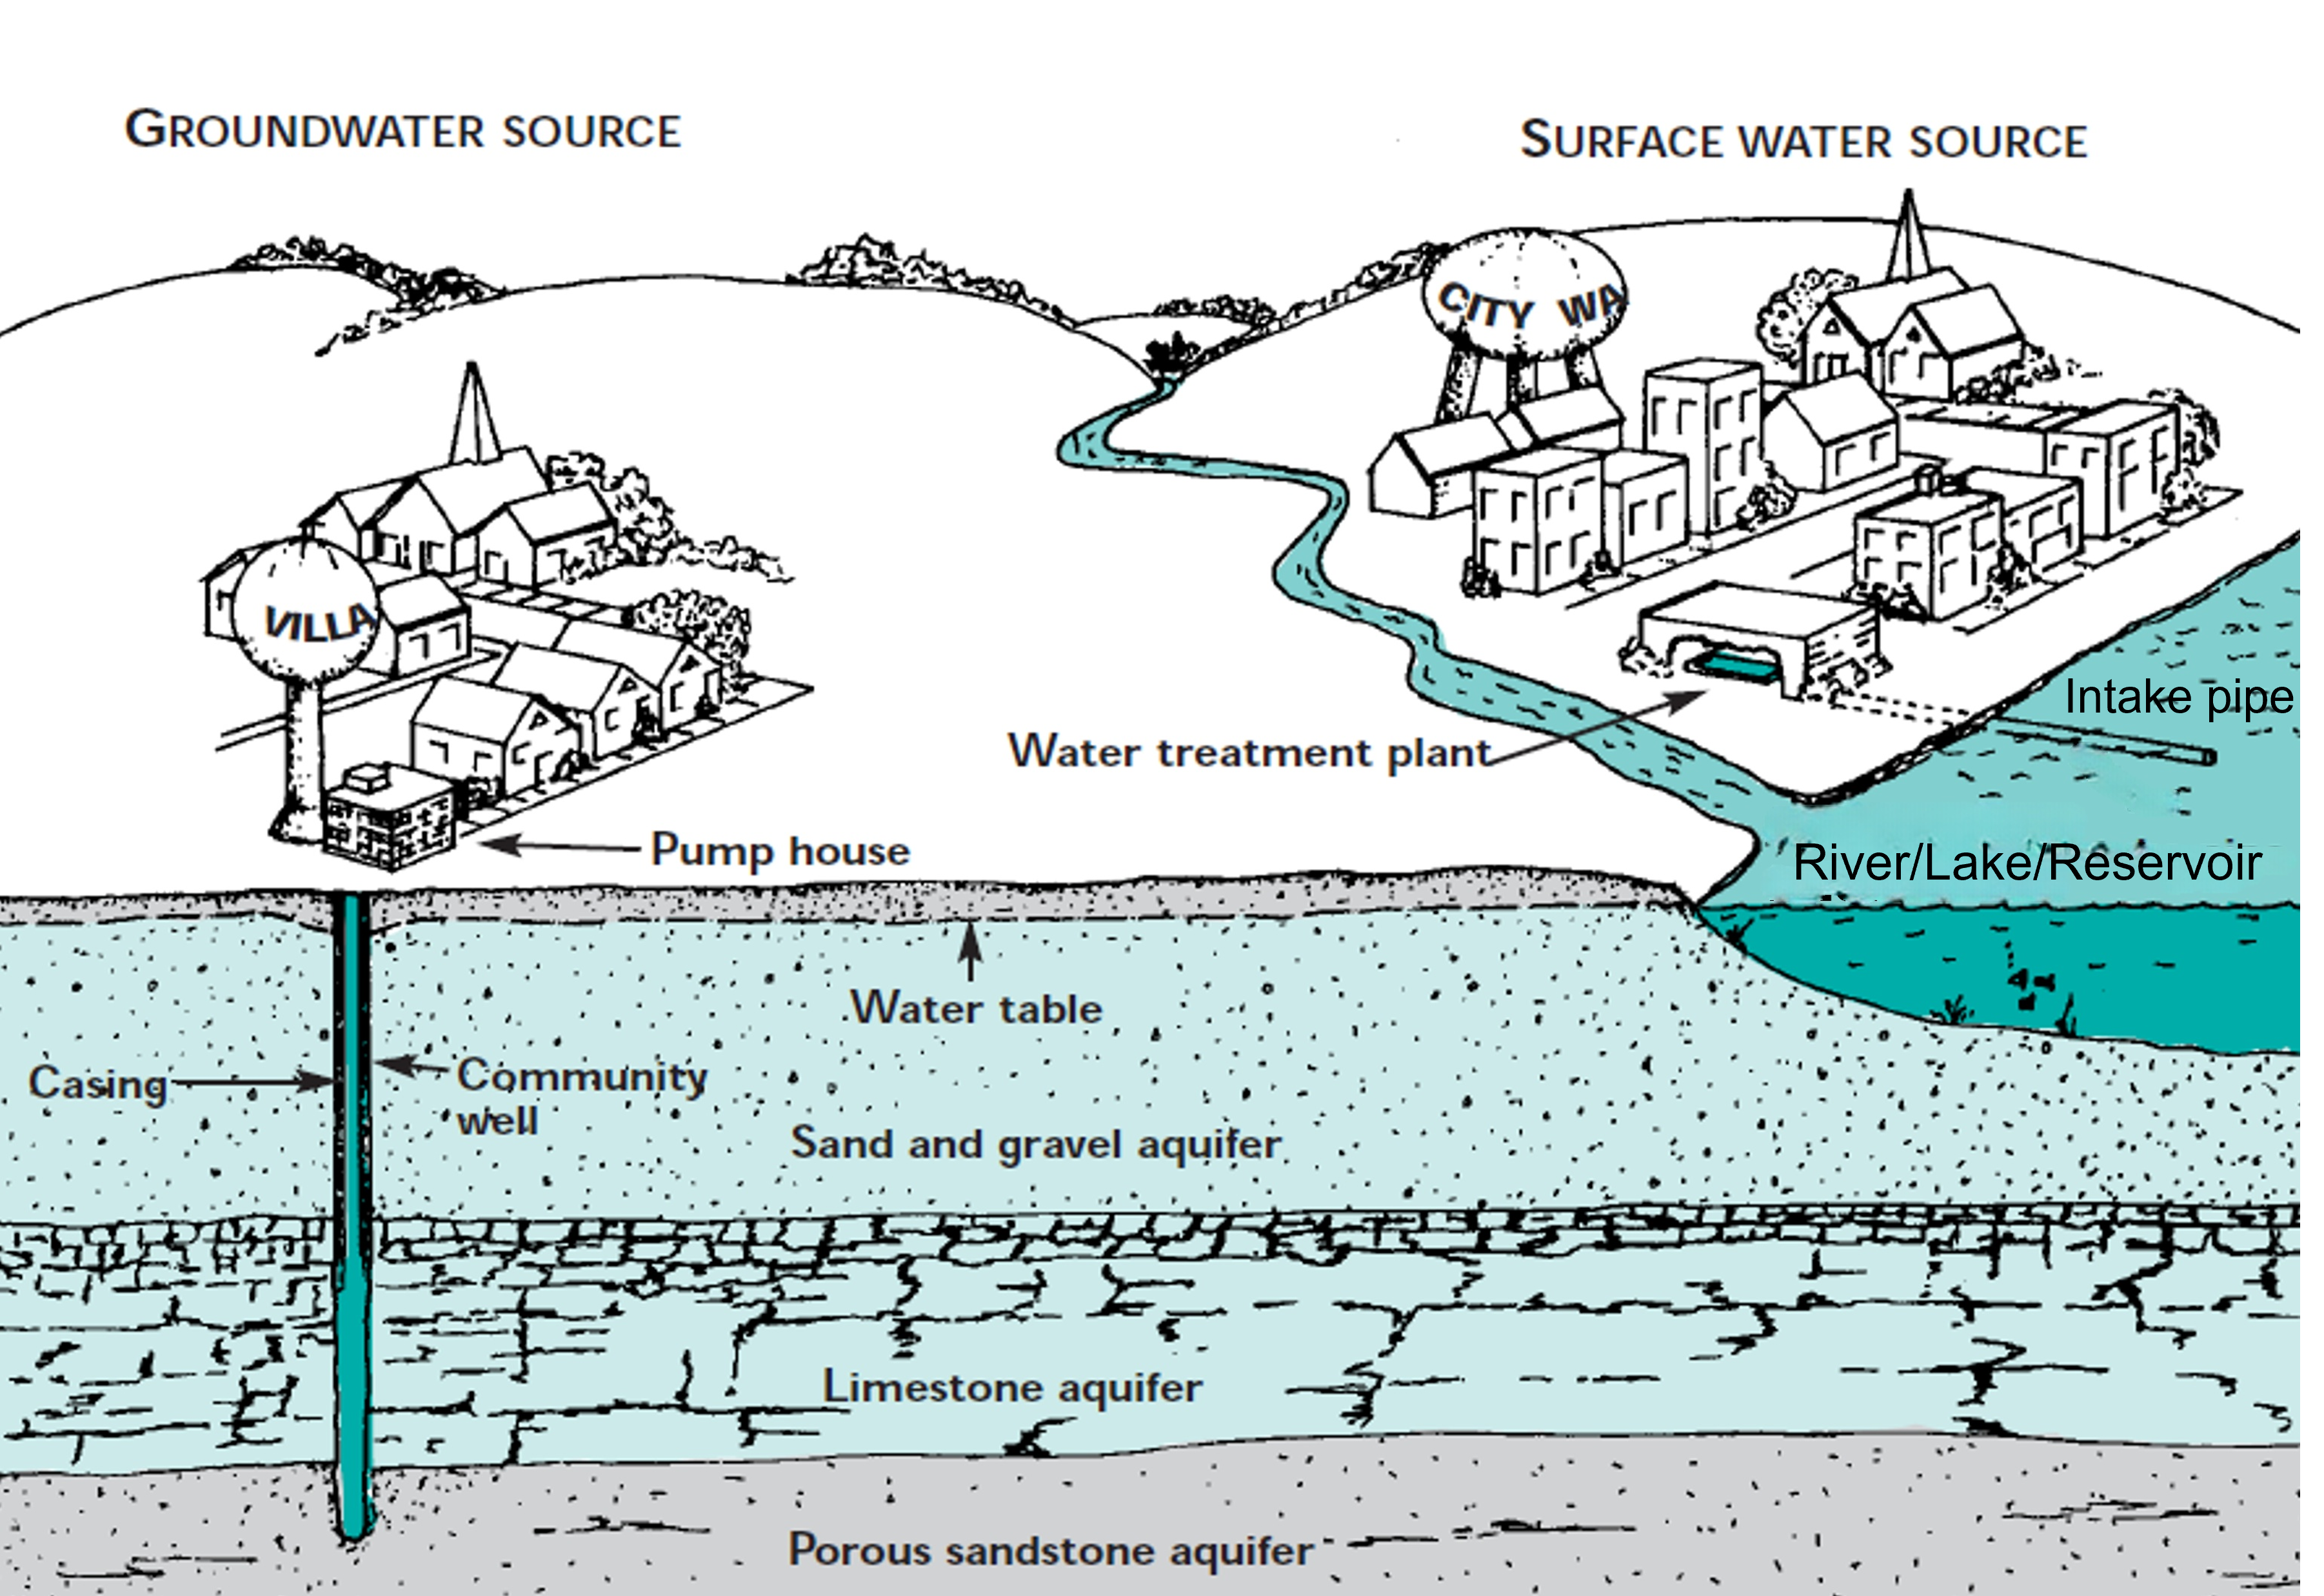
\includegraphics[scale=0.53]{WaterSources}\\
\captionof{figure}{Water supply sources}%\caption{}
\label{Water supply sources}
\end{center}
\end{figure}
\item Water sources include:
\begin{enumerate}
\item Surface water (for example, a lake, river, or reservoir)
\item Groundwater (for example, an aquifer)
\item Recycled water - also called reused water\\
\end{enumerate}
\end{itemize}
\begin{figure}[h!]
\begin{center}
\includegraphics[scale=0.3]{WaterSupplyIllustration1}\\
\captionof{figure}{Illustration of Southern California water supply systems} \label{Illustration of Southern California water supply systems}
\end{center}
\end{figure}

\begin{figure}[h!]
\begin{center}
\includegraphics[scale=0.4]{LosAngelesWaterSupply}\\
\captionof{figure}{Los Angeles area source water summary}%\caption{}
\label{Los Angeles area source water summary}
\end{center}
\end{figure}
\subsection{Groundwater}\index{Groundwater}
\begin{itemize}
\item Groundwater is the water found underground in spaces between sand, rock and soil. 
\item Groundwater is stored in aquifers - water-bearing formations underneath the surface that readily transmit water. 
\item \textbf{Aquifers} \index{Aquifer} are underground layers of very porous water-bearing soil or sand with enough groundwater that it can be pumped to the surface and used for drinking water, irrigation, industry, or other uses.
\item Water from precipitation, such as rain or snow, naturally filters through the soil, and is held within the aquifer. 
\item Groundwater can move through the aquifer and resurface through springs and wells.  The rate at which groundwater moves through an aquifer varies depending on the permeability of the layer.
\item Groundwater is extracted from aquifers via well pumping.
\item Groundwater moves from higher elevations to lower elevations and from areas of higher pressure to areas of lower pressure.
\item Groundwater is not stored in huge underground caverns, groundwater fills the pores of the various kinds of rocks that form the earth below us. \textbf{Hydrogeology} is the study of groundwater.
\item The presence of the groundwater depends largely on the geology of a specific area and the variable porosity of the upper portion of the earth’s crust. 

\item Access to groundwater is through:
\begin{enumerate}
\item \textbf{Wells} \index{Wells} - an ordinary well is essentially an a hole in the ground to access the water in the aquifer.
\item \textbf{Artesian Well} - as the groundwater moves in a aquifer, in certain areas of poor permeability, the water is pressurized.  In a well dug in this area, the water level will rise above the top of the aquifer and may even flow onto the land surface - {\textbf{flowing artesian well}}
\item \textbf{Springs} \index{Springs} - which is the flow of groundwater onto the earth's surface through a natural opening.  Springs occur when the contact between an upper aquifer and a lower aquitard intersects the ground surface
\begin{figure}[h]
\begin{tabular}{  m {8 cm}  m {8 cm} } 
\begin{center} \includegraphics[scale=0.6]{GroundWaterSpring} \end{center} & \begin{center}\includegraphics[scale=0.4]{Groundwater1} \end{center}\\
\begin{center} \textbf{Springs} \end{center} & \begin{center}\textbf{Groundwater} \end{center}\\
\end{tabular}\\
\end{figure}
\end{enumerate}
\item There are two general types of aquifers: confined and unconfined. \textbf{Confined Aquifers} \index{Aquifer!Confined and unconfined}have a layer of impenetrable rock or clay above them, while \textbf{Unconfined Aquifers} lie below a permeable layer of soil.
\item The layers of earth which hold the groundwater include a spectrum of layer with porous layer through which the groundwater could through easily in the downward direction, at one end of that spectrum to an \textbf{Aquiclude} which is a geological material through which zero flow occurs.
Then there is the \textbf{Aquitard} \index{Aquifer!Aquiclude, aquitard} in the middle, which is compacted layers of clay, silt or rock that retards the water flow.
\item The replenishment of aquifers by precipitation is called recharging \index{Aquifer!Recharging}. 
\item Aquifers naturally filter groundwater by forcing it to pass through small pores and between sediments, which helps to remove substances from the water. This natural filtration process, however, may not be enough to remove all of the contaminants.
\textbf{Safe yield} \index{Aquifer!Safe yield} is the maximum quantity of water which can be extracted from an aquifer, yet still maintain the supply unimpaired.
\item The \textbf{water table} is the surface of the water level in an unconfined aquifer at which the pressure is atmospheric.  The water table fluctuates due to recharge or outflow from the aquifer,
\item \textbf{Perched water table} is a small water body separated from the main groundwater by a relatively small impermeable stratum.
\item A \textbf{piezometeric surface or a potentiometric surface} \index{Aquifer!Piezometeric surface or potentiometric surface}is an imaginary surface to which the water level would rise if a piezometer - an  instrument used for measuring the pressure of groundwater, is inserted in a well drilled in a confined aquifer.  A piezometeric surface is the water table equivalent of a confined aquifer.
\item Groundwater can become depleted if used at a faster rate than it can be replenished. 
\item Groundwater can become contaminated when an excessive amount of pesticides and herbicides are sprayed on agricultural fields, septic tanks leak, or landfills are improperly lined or managed and toxic materials seep through the soil into the aquifer.
\item Groundwater can be found at nearly every point in the Earth's shallow subsurface to some degree, although aquifers do not necessarily contain fresh water.
\item Most land areas on Earth have some form of aquifer underlying them, sometimes at significant depths. In some cases, these aquifers are rapidly being depleted by the human population.
\item Many parts of the world are heavily dependent on groundwater due to low levels of rainfall.
\item The United States relies on groundwater for 23 percent of its freshwater needs.  In California, that number is significantly higher – groundwater provides nearly 40\% of the water used by California’s farms and cities, and significantly more in dry years.
\end{itemize}

\subsubsection{Water Wells}\index{Water wells}
\textbf{Background}
\begin{itemize}
\item A well is basically a hole in the ground, held open by a pipe (or casing) that extends to an aquifer.
\item A pump draws water from the aquifer for distribution through the plumbing system. 
\item Factors dictating the siting of a well include:
\begin{itemize}
\item Amount of water needed
\item Quality of available water
\item Meet minimum isolation distances required by state rules to ensure safety, and minimize any contamination potential.
\end{itemize}
\item The depth to which wells are constructed is determined by factors including:
\begin{enumerate}
\item depth to groundwater
\item groundwater quality, and 
\item geological conditions at the well site
\end{enumerate}
\end{itemize}
\textbf{Common well terms}\index{Wells!Well terms}:
\begin{itemize}
\item \ul{Static level} \index{Wells!Static level} is the water level in a well when the pump is not operating.
\item \ul{Pumping level} \index{Wells!Pumping level} is the water level in the well when it is producing.
\item Drawdown  \index{Wells!Drawdown} is the difference in elevations between the static level and the pumping level. The amount of water produced is approximately proportional to the drawdown.
\item \ul{Cone of depression}  \index{Wells!Cone of depression} is the depression in the water table formed as the pump draws down the water level.
\item \ul{Zone of influence} \index{Wells!Zone of influence} is the area included in the cone of depression.  Any contamination in this zone will be drawn into the well.
\item \ul{Radius of influence} \index{Wells!Radius of influence} is the farthest distance from the well that the cone
of depression affects the water table.
\item \ul{Specific capacity} \index{Wells!Specific capacity}is the relationship between the yield of a well and the amount of drawdown in the well. It can be expressed as a ratio of the yield, in terms of gallons per minute, to the drawdown in feet. A well producing 100 gpm with a drawdown of 20 feet would have a specific capacity of 5 gpm per foot of drawdown.






%    \begin{minipage}{0.5\textwidth}
%        \centering
%        \includegraphics[width=0.75\linewidth, height=0.25\textheight]{WellDrawdownCalc}
%        \caption{Drawdown calculations}
%        \label{fig:prob1_6_1}
%    \end{minipage}








%\begin{figure}[h!]
%\begin{center}
%\includegraphics[scale=0.7]{Welldesign}
%\caption{Well construction}
%\end{center}
%\end{figure}
%\begin{figure}[h!]
%\begin{center}
%\includegraphics[scale=0.5]{Well}
%\caption{Well calculations}
%\end{center}
%\end{figure}
\item \ul{Recovery time} \index{Wells!Recovery time}is the amount of time required for the aquifer to stabilize at its static water level once pumping has stopped.
\end{itemize}
\begin{figure}[!htb]
    \centering
    \begin{minipage}{0.8\textwidth}
        \centering
        \includegraphics[width=0.6\linewidth, height=0.25\textheight]{WellTermsGraphic2}
        \caption{Well terms}
        \label{Well terms}
    \end{minipage}%
    \end{figure}


\textbf{Well types} \index{Wells!Well types}
\begin{itemize}
\item Wells are classified by method of construction of the well.
\item Well types \index{Wells!Types of wells}include:
\begin{itemize}
\item Dug wells \index{Wells!Types of wells!Dug,driven,drilled wells}:  These wells are typically:
\begin{itemize}
\item large diameter
\item 10-30 ft deep
\item hand-dug to the top layer of the aquifer.  
\item lined with stone or bricks
\end{itemize}
Dug wells levels fluctuate with seasonal variation of water table and has a high risk of contamination from nearby land activities.

\item Driven wells:  These wells are for reaching shallow waters about 30-50 feet deep and are made by driving a small diameter pipe.  Although the well is cased, it has a moderate to high evel of risk of contamination from nearby land activities.

\item Drilled wells:  Drilled well is the most common type of well used by public water systems.  These wells are constructed using a rotary-drilling machine and are hundreds of feet deep.  These wells have a continuous casing, which is commonly six-inches in diameter.  These wells are ideally suited to deep water bearing formations where larger yields are available. This type of well, when properly constructed offers good protection against contamination from the surface.
\end{itemize}

\end{itemize}

\textbf{Well Construction} \index{Wells!Well construction}\\
Elements of well construction include:\\
\begin{itemize}
\item \ul{Borehole} \index{Wells!Wells construction!Borehole} is the narrow shaft drilled to extract water from the aquifer.
item \ul{Well casing} \index{Wells!Well construction!Well casing} is the watertight plastic  or steel tube lining of the borehole.  It is generally 4-6" diameter and it is primarily to protect the borehole from caving in and to prevent surface water from entering the well.  The casing should extend at least 6 to 12 inches above the
well pad, depending on whether the well is located in a well house or out in the open, to prevent standing water from entering the well.
\item \ul{Well screen} \index{Wells!Well construction!Well screen}  is installed on the end of a well casing.  It supports the bore hole, and it reduces the amount of sand that enters the casing and the pump.
\item \ul{Gravel packer} \index{Wells!Well construction!Gravel packer} is a layer of gravel placed around the screen to reduce the amount of fine material from entering the well through the screen.  The gravel packing is usually three times the diameter of the well screen or a minimum of 4" thick.
\item \ul{Grout} \index{Wells!Wells construction!Grout} is cement or bentonite packing around the well casing to protect the well from surface water.  The grout is applied continuously from the surface upto the bottom where the borehole passes into the impermeable layer or upto the gravel packer.
\item \ul{Ground seal} \index{Wells!Well construction!Ground seal}is typically a reinforced concrete slab. This concrete is usually connected to the grout that extends down the well.
\item \ul{Sanitary seal}\index{Wells!Well construction!Sanitary seal} it seals the top of the casing and its primary function is to prevent well contamination.  The type of seal varies depending upon the type of pump being used.  For a well using a submersible pump, the sanitary seal is typically composed of a rubber-like material
placed between two pieces of metal. When bolts are tightened on the sanitary seal, the rubber is compressed and expands to seal against the casing and the pump discharge pipe.
\begin{figure}[h!]
\begin{center}
\includegraphics[scale=0.6]{Welldesign}
\caption{Well construction}
\label{Well construction}
\end{center}
\end{figure}
\end{itemize}
\subsection{Groundwater Under the Direct  Influence  of  Surface  Water}\index{Groundwater under the direct  influence  of  surface  water (GWUDISW)}
\begin{itemize}
\item Groundwater under the direct  influence  of  surface  water (\textbf{GWUDISW}) is the water which may be subject to contamination with pathogenic organisms from surface waters. 
\item GWUDISW is defined as:\\
Any water beneath the surface of the ground with significant occurrence of:\\
\begin{itemize}
\item Insects 
\item Other macroorganisms
\item Algae
\item Large diameter pathogens such as Giardia lamblia
\end{itemize}
\vspace{0.3cm}
or as:\\
\begin{itemize}
\item Any water beneath the surface of the ground with significant and relatively rapid shifts in water characteristics such as:
\begin{itemize}
\item Turbidity
\item Temperature
\item Conductivity, or
\item pH
\end{itemize}
that closely correlates to climatological or surface water conditions.     
\end{itemize}
\end{itemize}

\subsection{Surface water}\index{Surface water}
\begin{itemize}
\item Surface water is water that is open to the atmosphere and results from overland flow. It is also said to be the result of surface runoff. These are two ways of saying the same thing.
\item Examples of surface water include:
\begin{itemize}
\item Streams, Rivers, Lakes
\item Man-made impoundments - Reservoirs
\item Wells drilled next to or in a stream or river
\item Rain catchments
\end{itemize}
\item Surface waters are classified as either:  running waters which include streams, rivers and brooks; and quiescent waters which include lakes and reservoirs.
\
\item  A lake is where surface-water runoff (and maybe some groundwater seepage) have accumulated in a low spot, relative to the surrounding countryside.  Whereas a reservoir is a man-made lake that is created when a dam is built on a river. 
\item The exposure of surface waters to the atmosphere results in exposure to precipitation events, surface water runoff and contamination with micro and macroorganisms resulting from activities in their surrounding areas.

\item Changes in weather cause the natural flow of streams and rivers to vary greatly with time. Periods of excess flows and valley flooding may alternate with low flows or droughts.
\item  The role of water-storage reservoirs, also known as impoundments is to store water during periods of higher flows, thus preventing flood disasters, and then permit gradual release of water during periods of lower flows. 

\item Lakes and reservoirs can be classified into three categories \index{Surface water!Lakes and reservoirs classification} based upon their nutrient content:
\begin{itemize}\index{Eutrophic} \index{Mesotrophic} \index{Oligotrophic}
\item Eutrophic - rich in nutrient
\item Mesotrophic - moderate amount of nutrient 
\item Oligotrophic - little or no nutrient
\end{itemize}
\item In many locations, as the water temperatures decrease with increasing water depth, thermal stratification \index{Lake thermal stratification} - formation of distinct thermal layers, of lakes and reservoirs occur due to temperature related density changes which prevents the vertical mixing of water. 
\begin{enumerate} \index{Epilimnion} \index{Thermocline} \index{Hypolimnion}
\item Epilimnion - Suface layer of warm, light water (mixed by wind)
\item Thermocline or Metalimnion- Middle layer with rapidly changing temperature
\item Hypolimnion - Lowest layer of coldest and densest water. Hypolimnion usually has depletion of dissolved oxygen (DO) leading to fish kills for fish living at that depth.	·
\end{enumerate}

\begin{figure}
\begin{center}
\includegraphics[scale=0.5]{ReservoirStratification}\\
\captionof{figure}{Lake/reservoir stratification}%\caption{}
\label{Lake/reservoir stratification}
\end{center}
\end{figure}
\item Destratification \index{Destratification} - can be natural by change in weather or by means such as aeration or mechanical agitation and mixing.
\item Lake turnover \index{Lake turnover}- During autumn and winter, top layer of water gets colder and denser and
sink to the bottom, water from bottom comes to the top causes the bottom sediments to be stirred	causing high turbidity in the water. It can also cause the heav metals (such as mercury and lead from the bottom of the reservoir become dispersed in the water.

\item Thus, water intakes are located at various levels in the reservoir to get the best possible quality of raw intake water possible at different times of the year.

\end{itemize}

\subsection{Advantages and disadvantages of surface water vs groundwater }\index{Advantages and disadvantages of surface water vs groundwater }
\begin{itemize}
\item Advantages of surface water with respect to groundwater:
\begin{itemize}
\item It is easily located. It takes no sophisticated equipment to find a surface water source.
\item In many parts of the US, considerable data is available on quantity and quality of existing surface water supplies.
\item Surface water is generally softer than groundwater, which makes treatment much simpler.
\end{itemize}
\item Disadvantages of surface water with respect to groundwater:
\begin{itemize}
\item Surface waters can be easily contaminated with microorganisms that cause waterborne diseases and chemicals that enter the stream from surface runoff and upstream discharges.
\item The turbidity of a surface water source often fluctuates with the amount of precipitation. Increases in turbidity increase treatment cost and operator time.
\item The temperature of surface water fluctuates with the ambient temperature. This makes it difficult to produce consistent water quality at a water treatment plant.
\end{itemize}
\item Advantages of groundwater with respect to surface water:\\
\begin{itemize}
\item Groundwater is not as easily contaminated as surface water.
\item The quality of groundwater, while not always as good as would be preferred, is stable throughout the year.
\item Groundwater sources are generally lower in bacteriological count than surface water sources.
\item Groundwater is available in most locations throughout the continental US and Alaska.
\end{itemize}
\item Disadvantages of groundwater with respect to surface water:\\
\begin{itemize}
\item Groundwater usually contains more minerals than surface water, including increased levels of hardness. Because groundwater is in contact longer with minerals, there is more time to bring them into solution.
\item Removal of groundwater normally requires a pump, thus increasing operation cost.
\item Groundwater is more susceptible to long-term contamination from fuel spills.
\item Groundwater supplies often have high levels of iron and manganese, thus increasing treatment cost and/or causing stains on plumbing and the clothing of customers.
\item Wells in the coastal areas are subject to salt water intrusion into the aquifer
and well. This contamination is difficult to predict and costly to treat.
\item Once a groundwater source is contaminated, it is difficult for it to recover. There is no easy way to remove the contaminants. Sources of contamination can be hidden from sight.
\end{itemize}
\end{itemize}
\begin{figure}
\begin{center}
\includegraphics[scale=0.5]{WaterContamination}\\
\captionof{figure}{Sources of water contamination}%\caption{}
\label{Sources of water contamination}
\end{center}
\end{figure}
\subsection{Recycled water}\index{Recycled water}
\begin{itemize}
%\item Within the Water Cycle, there are many subcycles which can be regional or local.
%\item One such cycle is the local cycle which involves water use and reuse.\\
%\begin{figure}
%\includegraphics[scale=0.2]{Test4}\\
%\captionof{figure}{Water Use - Reuse Cycle}%\caption{}
%\end{figure}
\item Water reuse (also commonly known as water recycling or water reclamation) reclaims water from a variety of sources then treats and reuses it for beneficial purposes such as agriculture and irrigation, potable water supplies, groundwater replenishment, industrial processes, and environmental restoration.
\item Water reuse can provide alternatives to existing water supplies and be used to enhance water security, sustainability, and resilience.

\item Unplanned or de facto reuse refers to situations in which a source of water is substantially composed of previously-used water. An example of unplanned water reuse occurs when communities draw their water supplies from rivers, such as the Colorado River and the Mississippi River, that receive treated wastewater discharges from communities upstream.
\end{itemize}

\section{Water rights in California}\index{Water rights}
\begin{itemize}
\item If one takes water from a lake, river, stream, or creek, or from underground supplies for a beneficial use, California law requires that person to have a water right. The term “beneficial use” can refer to agricultural, mining, urban, industrial, or environmental uses.
\item In California, water rights law is administered by the State Water Resources Control Board (often called simply the State Water Board). 
\item A water right holder is entitled to a “reasonable” amount of water, which not only considers the purpose for which the water is being used but also the relative consumption of the water with regard to other water users in the system.
\item Two types of water are recognized by law in water with regard to the law: groundwater and surface water.
\item Groundwater is considered a local supply and there is little state regulation of its use,and consequently a state water right permit is not required for use of this water.
\item Primarily, landowners in California are entitled to pump and use a reasonable amount of groundwater from a basin underlying their land to put it to a beneficial, nonwasteful use.
\item The use of surface water is subject to state laws and regulations that control its development and use.
\item Most common surface water rights include:
\begin {enumerate}
\item Riparian rights \index{Water rights!Riparian rights}:\\
\begin{itemize}
\item Riparian rights are rights to the “reasonable and beneficial use of water on land that is adjacent to a watercourse - a lake, river, stream, or creek. 
\item A riparian right allows the landowner to take as much water as can be reasonably and beneficially used on the riparian property. 

\item Riparian owners must share with other riparian owners along the same water body, and they cannot waste water or unreasonably affect public trust resources. 

\end{itemize}

\item{Appropriative Rights} \index{Water rights!Appropriative rights}:\\
\begin{itemize}
\item Appropriative water rights are legal rights to use water from a water source, such as a river or stream, for beneficial purposes.
\item Someone who takes water for use on non-riparian land or who uses water that would not be there under natural conditions on riparian land, appropriates water.
\item These rights are typically granted based on the principle of "first in time, first in right," meaning that the first person or entity to beneficially use the water for a specific purpose has priority over later users. 
\item Appropriative water rights are common in regions where water is scarce and are often subject to regulations and permitting processes to ensure fair and sustainable allocation of water resources.
\item Water right permits and licenses issued by the State Water Board are appropriative water rights.
\item Appropriative water may be stored for later use, or held for diversion and beneficial use.
\end{itemize}

\item Prescriptive Rights \index{Water rights!Prescriptive rights}:\\
\begin{itemize}
\item A prescriptive right is a right that is acquired through adverse possession of someone else’s water right. It is similar to a “squatter’s right” to land.
\item Prescriptive rights originated in the context of conflicts between competing riparian users.
\end{itemize}

\end{enumerate}
\end{itemize}
